%=======================================================================================%
\chapter{Review of Cystic Fibrosis and The Molecular Basis of its Treatment}
\label{chap:cftr}
\chapquote{Because of what's inside me; Because of my genes.}{-Bob Flanagan \cite{dick1997}.}
\newpage
%Authors note:
% We begin with a breif overview of the disease Cystic Fibrosis as it is the main motiation for this project. A horrendous disease for which we will hopefully soon find a cure.

%Clinical outcomes are a chronic illness which affects multiple organ systems and every aspect of a patient's life. 
	%physical therapy, pancreatic sufficiency, ongoing discovery of chronic issues. Much to do. 


% The cause of the disease is CFTR misfunction.
       % CFTR function overview

% CFTR modulators act to restore its function. 
	% patients with rare genotypes cant access modulators.

This thesis primarily focusses on the molecular causes of Cystic Fibrosis. In subsequent chapters we will use Molecular Dynamics (MD) to determine what kind of defect rare mutations cause to CFTR, the gene whose mutation causes CF. We do this with the goal of understanding what kind of treatments they might respond to. Given the importance of the CFTR protein system to this work, we will look at its structure and dynamics in detail in this chapter. However, to understand the motivation for these studies, we will first review some of the medical literature surrounding the disease itself. 

In previous chapters we always worked upward. In chapter \ref{chap:methods} I showed how we can begin from Schr\"odinger's wave equation to understand biomolecular systems. This was to give an example of the philosophy I outlined in chapter \ref{chap:introduction}, taking abstract formalisms and integrating them to model macroscopic biophysical phenomenon. By contrast, in this chapter we will work downward, beginning with the reality of living with this disease before we look at its molecular cause and its treatment. I have taken particular care to begin this chapter with a discussion of the clinical outcomes of the disease we are studying, so we do not lose sight of our goals in studying biophysics. 

When one trains to practice medicine they are taught how to conduct themselves ethically, with their patients best interests at heart \cite{hajar2017}. I have had no such training and I knew I was missing something by studying this disease so impersonally \cite{foucault1994}. In the 20th century, physicists often participated in political and moral discourse, not always for the better \cite{frank1993, gottfried1999, global2009, rhodes1986, aaronson2008, berger2016, vonneumann_britanica}. Should we wish to embark on the enterprise of studying biophysics we have a responsibility to also study how to do it ethically. Thankfully, many of these important questions have been pondered for some time by philosophers and the reader is encouraged to seek texts on bioethics and also ethics in the use of artificial intelligence \cite{buchanan2000, taneri2011, genome_editting_guildelines_2017, muller2021, bostrom2014}. These considerations will become increasingly important as biophysics advances. As biophysical techniques increase in capacity, so too does their capability for misuse \cite{mallapaty2022, urbina2022}. 

%On this somewhat somber note, we will now take a brief look at what it is like to live with Cystic Fibrosis.

%We will then analyse the root cause, mutations to the Cystic Fibrosis transmembrane Conductance Regulator (CFTR). In chapter \ref{chap:conclusion} we will use much of the knowledge gained in this chapter to think about where we can direct future studies to help treat the root cause of Cystic Fibrosis. 



\section{Clinical Realities of Living with Cystic Fibrosis}
Cystic Fibrosis (CF) is the most common fatal genetic condition in Caucasian populations. Over 162 000 people are estimated to be afflicted globally, with a significant proportion living undiagnosed \cite{hammoudeh2021,guo2022}. Even with decades of research there is no known cure for CF and those patients have an average below 50 \cite{mcbennett2022}. Management of disease symptoms also bears significant financial and emotional costs to patients and their families \cite{vangool2013, page2022}. From a cellular perspective the symptoms of the disease are due to the inability of certain cells to regulate their salt content. 

\begin{figure}
	\label{CF_summary}
	\begin{center}
	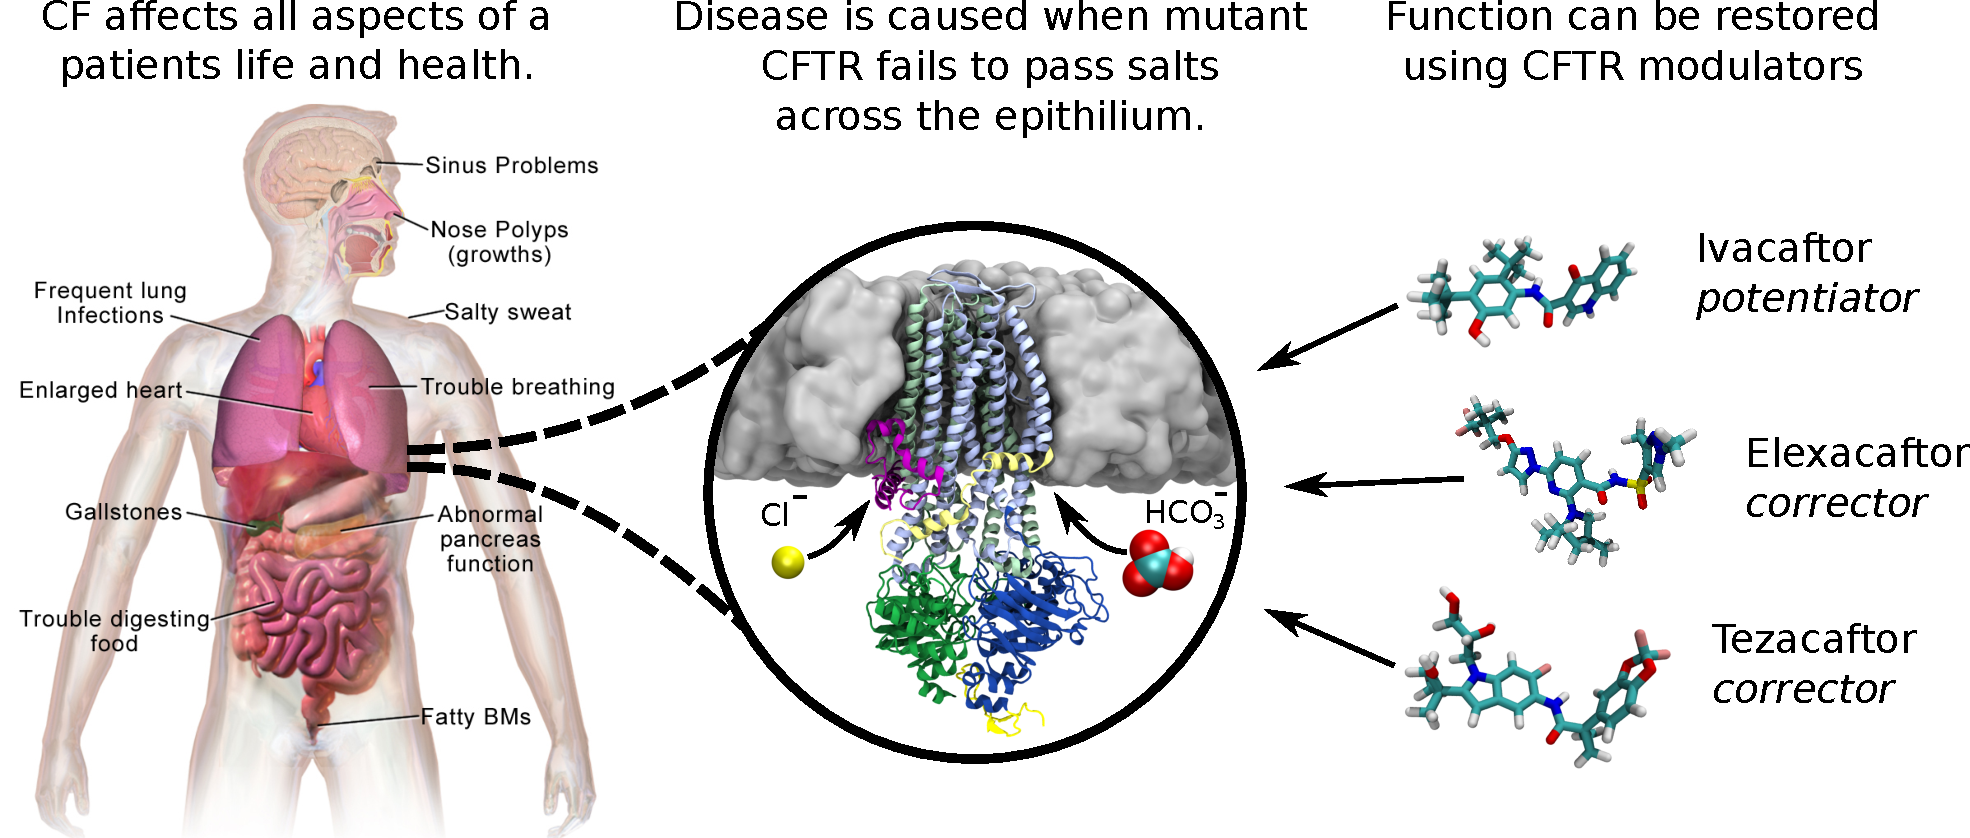
\includegraphics[width=1\textwidth]{figures/cf_summary_fig.pdf}
	\end{center}
	\captionsetup{singlelinecheck = false, justification=raggedright}
	\caption[Cystic Fibrosis is a Debilitating Disease Whose Cause is Genetic] {\textbf{Cystic Fibrosis is a Debilitating Disease Whose Cause is Genetic}}{Cystic Fibrosis effects several major organ systems, affecting all aspects of a patients life. The cause of the disease is genetic, when a defective copy of an anion channel, CFTR, are inherited from each parent epithelial cells cannot pass chloride or bicarbonate ions, leading to a buildup of salts inside epithelial cells. In recent decades, small molecule drugs have been discovered which act directly on CFTR to restore its function. This thesis seeks to understand what kind of defects these drugs are capable of rescuing. We find that they are likely to rescue a wide range of defects.} 
\end{figure}

All organs of the body are lined by membranes called epithelium, which protects them from trauma and fection. The most acute symptoms of CF are due to the dehydration of these epithelium several organs. Of most concern is the epithelium in the lungs. When dehydrated, fine, motile structures called cilia, which line the epithelium collapse, rendering them unable to ``beat" and clear pathogens \cite{boucher2007}. Simultaneously, this dehydration causes the mucus which naturally lines the epithelium to thicken, as osmotic pressure leaches moisture away from it. 

This thickened mucus has two pathogenic effects. Firstly, the stationary mucus allows bacterial colonies to infect the lungs, this can degrade lung function and remains one of the most troublesome chronic complications in CF patients \cite{}. Secondly, and more acutely, this thick mucus inhibits the normal function of several organ systems. For example, the pancreas is not able to secrete digestive enzymes into the body and the lungs struggle to absorb oxygen. A patient whose pancreas does not produce sufficient enzymes to digest nutrients is referred to as ``pancreatic insufficient" (PI). This is an important determinant in the severity of disease and their quality of life \cite{}.

Much of the increased life expectancy of CF patients has been due to the improved management of this mucus and the populations of bacterium infecting it \cite{}. Patients often undergo hours of physical therapy each day to help them clear this mucus from their lungs \cite{zotero-3683}. Inhalation of a saline solutions may also help relieve symptoms, as this draws moisture out of the epithelial cells by counteracting the pathogenic osmotic pressure gradient \cite{wark2018}. 

CF patients struggle to intake nutrients due to the build up of mucus in the ducts of their pancreas and large intestines. This leads to CF related diabetes which afflicts roughly half of adults with CF \cite{Kayani2018}. Patients to avoid and manage this complication patients are often administered digestive enzymes and must adhere to a specific diet. 

Interestingly, as patients are living longer, we are discovering more disease complications, such as bone disorders, meaning there is much clinical work to be done as managing CF becomes a life-long rather than an acute condition \cite{stalvey2013}. 

\begin{figure}
	\label{CF_life_expectancy}
	\begin{center}
	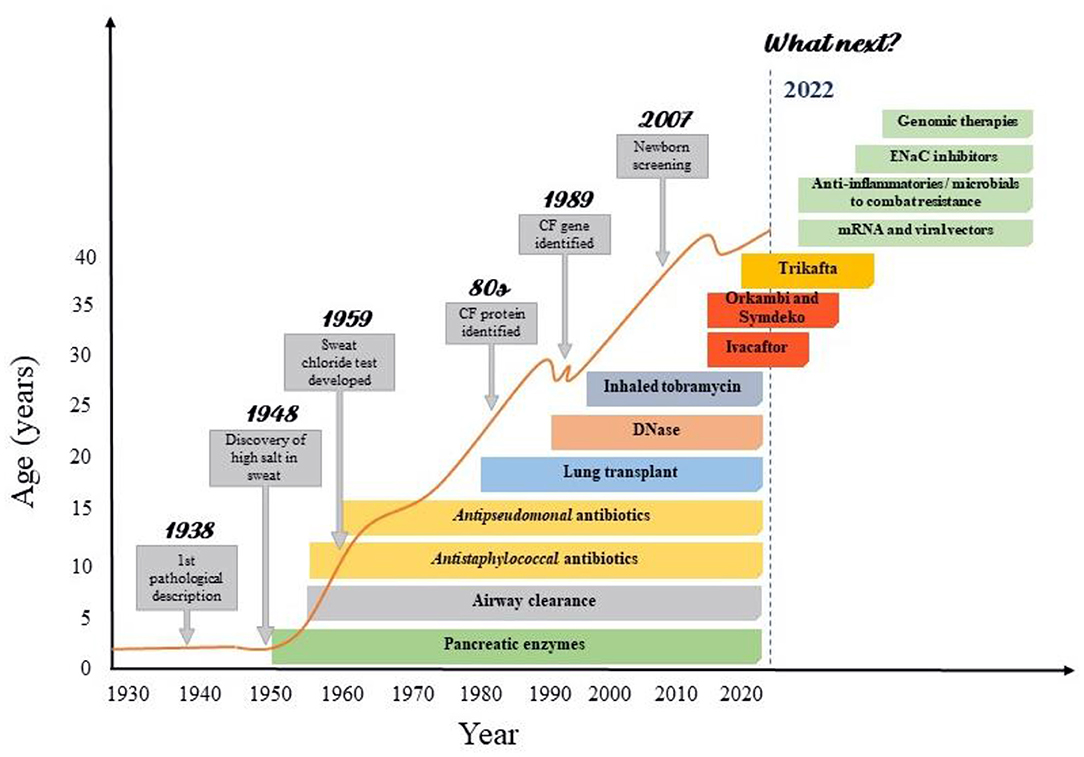
\includegraphics[width=0.7\textwidth]{figures/CF_life_expectancy.png}
	\end{center}
	\captionsetup{singlelinecheck = false, justification=raggedright}
	\caption[CF Clinical Progress] {\textbf{CF Clinical Progress}}{Life expectancy of CF patients correlates highly with translational research. As CF becomes a chronic condition patients will likely undergo a combination of more and more advanced therapies. Source \cite{garcia2022}} 
\end{figure}

Patients with CF struggle to lead a normal life. The gradually degrading lung function is nearly universally the cause of death in patients with cystic fibrosis \cite{}. The most common biomarker for tracking disease progress is known as FEV1\%, which stands for Forced Expiratory Volume in 1 second. It is a measure of the volume of air a patient is able to expel in one second, compared to their total lung capacity.

Although beginning this chapter with a discussion of clinical might seem out of place compared to the rest of previous chapters it is important to remember why we are doing the difficult work of biophysics. It is important, and physicists have a unique perspective, a capacity to do good which has historically been missing from the study of medicine. 

\section{The Misfunction of CFTR causes CF}

The primary cause of the disease Cystic Fibrosis (CF) is the malfunction of a chloride channel, the Cystic Fibrosis Transmembrane Conductance Regulator (CFTR). This ion channel is a member of the ABCC subfamily of ABC transporters, designated ABCC7. This channel is unique amongst this family because it is not generally considered an active transporter but something of a low conductivity channel or a "weak pump" \cite{linsdell2018}.

\begin{figure}
	\begin{center}
	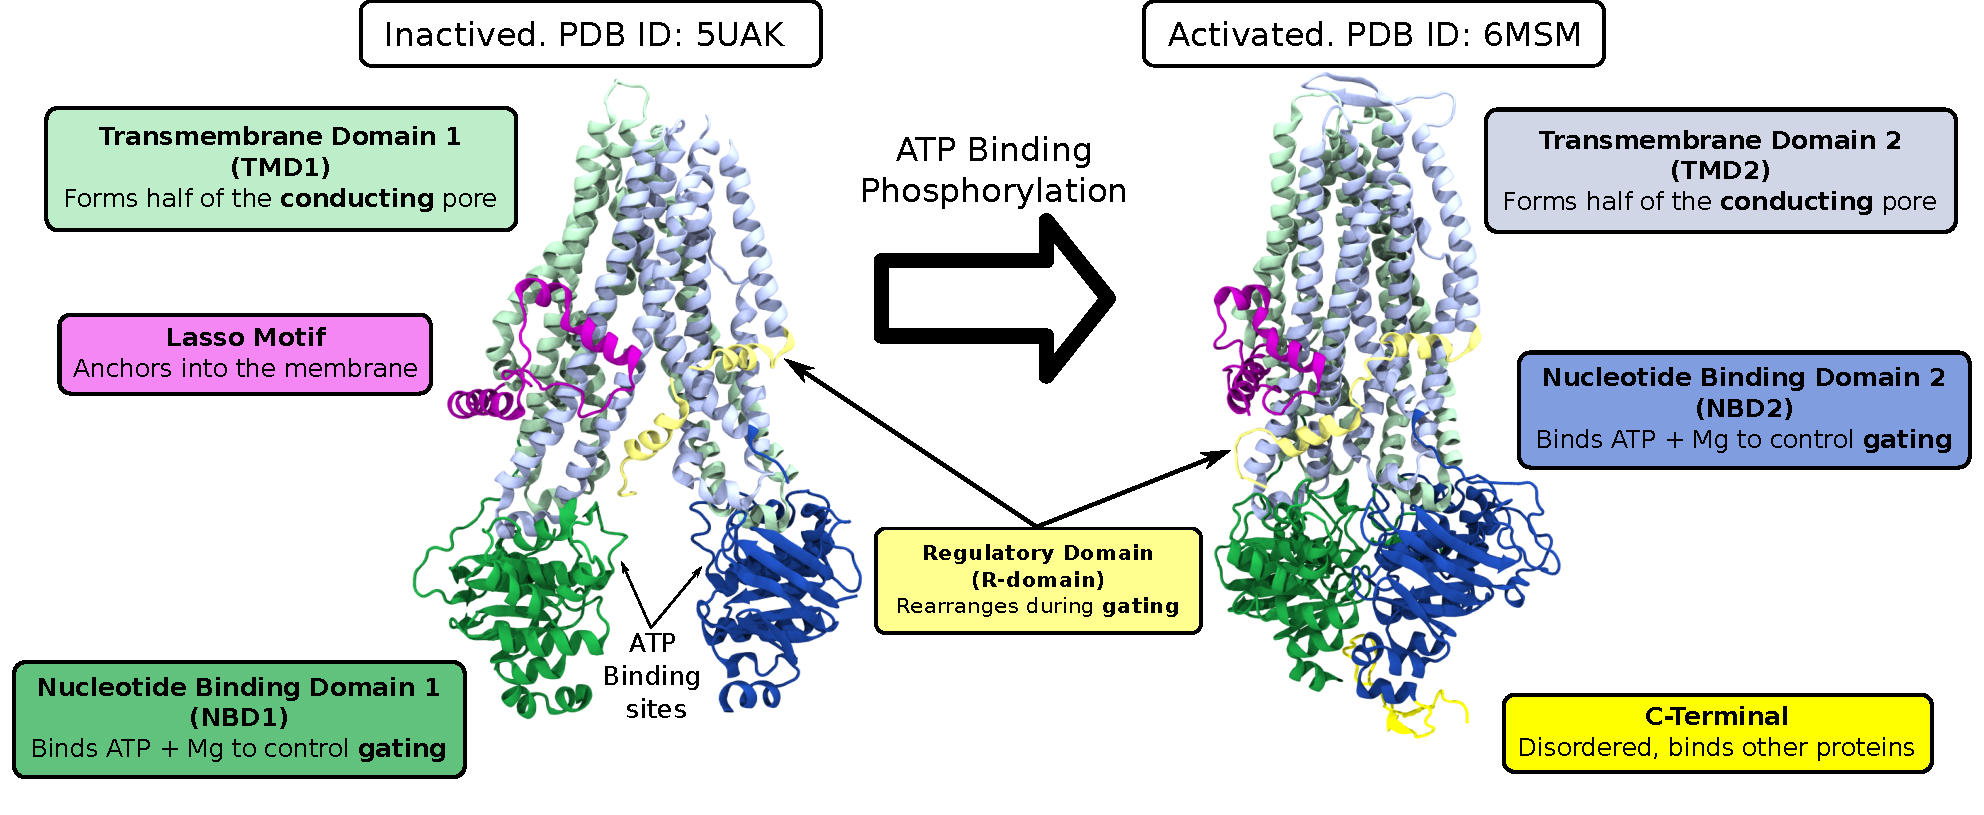
\includegraphics[width=\textwidth]{figures/CFTR_structure.pdf}
	\end{center}
	\label{CFTR_structure_domains}
	\captionsetup{singlelinecheck = false, justification=raggedright}
	\caption[CFTR Structure] {\textbf{CFTR Structure}}{There are currently two resolved human CFTR structures. The inactivated state is neither phosphorylated nor bound to ATP. Observe how the NBDs are far apart and the TMDs are not parallel, forcing a constriction near the top of the protein which does not allow the passage of ions. By contrast, the activated structure is abound to ATP at both sites, bringing the TMDs into a parallel configuration where they are able to form a pore. There are unresolved questions as to whether CFTR may conduct chloride in this conformation which we will analyse in chapter \ref{chap:opening}.} 

\end{figure}
CFTR is composed of one chain with pseudo-symmetric structure, the protein is well organised into 7 domains \ref{CFTR_structure_domains}. In the order of their primary structure they are: 
\begin{enumerate}
	\item The Lasso motif (AA 1-68). Anchors into the membrane and serves as an interaction hub with protein partners such as syntaxin and filamin which are important in cellular trafficking \cite{cormet-boyaka2002, naren1998, thelin2007} as well as WNK1 which plays a role in bicarbonate selectivity \cite{kim2019}.
	\item Transmembrane Domain 1 (TMD1 AA 69-376). This domain forms half of the chloride conducting pore and importantly, TM1 and TM6 in this domain form the extracellular end of the pore for anion permeation \cite{linsdell2006, linsdell2022}.
	\item Nucleotide Binding Domain 1 (NBD1 AA 377-629). One of the ATP binding sites, this domain has a dense concentration of disease causing mutations, including the most common mutation $\Delta F508$ \cite{cftr2}.
	\item Regulatory Domain (R-domain AA 630-855). A disordered domain containing up to 11 phosphorylation sites\cite{mihalyi2020}. In the inactivated conformation a helical segment of this domain wedges between the TMDs. Upon binding of PKA and phosphorylation the wedge relocates to a location just below the R-domain. The identity of a fragment of the R-domain is analysed in detail in chapter \ref{chap:I37R}. The kinetics of this domain is important to the overall function of CFTR \cite{ostedgaard2000, mihalyi2020}. 
	\item Transmembrane Domain 2 (TMD2 AA 856-1168). This domain forms the other half of the chloride conducting pore. There is ongoing controversy over the structure and function of TM8 the function of CFTR \cite{hegedus2022, liu2019}.
	\item Nucleotide Binding Domain 2 (NBD2 AA 1169 - 1450). Home to the conserved Q-loop, which plays an important role in the binding of ATP in ABC transporters \cite{ivey2020, zolnerciks2014, dong2015}.
	\item C-terminus (NBD2 AA 1451 - 1480). This structure is natively disordered but it serves as an interaction hub in WT-CFTR, anchoring CFTR to other proteins through its PDZ binding domain \cite{moyer1999, cushing2008}. 

\end{enumerate}


%CFTR is distinguished by a regulatory region known as the R-domain (residues 645-845) which links NBD1 to TMD2. This region acts to lock the channel in the closed state by wedging itself between the TMDs and dislodging when any one of 3 sites are phosphorylated \cite{mihalyi2020}. In experimentally determined structures of human CFTR the secondary structure of a section of the R-domain but not at high enough resolution to determine the identity of individual side chains \cite{zhang2018, zhang2016}. Further secondary structure information can be found through experiments with NMR \cite{Baker2007}.

Previous computational studies of CFTR have been used homology models based on the phosphorylated zebra fish protein PDBID:5W81 \cite{zhang2017a}. These have yielded interesting results but the sequence similarity between human and zebra fish CFTR is only 55\% \cite{}. For a protein structure where a single amino acid mutation leads to malfunction, more precision can only help. Additionally, the activity of CFTR correctors is not conserved in mutant zCFTR \cite{laselva2019}. In order to do precision medicine we need precision structures. 

An open state of the channel has been proposed by combining both the zebra fish homology model and the fully outward facing conformer of a bacterial ABC transporter Sav1866 \cite{Hoffmann2018}. Although this model has several characteristics expected of the open channel, such as the critical R352-D993 salt bridge, it lacks a salt bridge between R104-E116. In experiments, these residues could be replaced by cysteines and the channel would still function. However, when reducing agents were added to the system the channel lost its ability to open fully. This indicates that in the oxidised environment the C104-C116 cysteines formed a disulfide bridge but its breaking upon exposure to reducing agents caused a loss of function in the channel. This indicates that in the WT channel R104-E116 form a stable salt bridge. 

This salt bridge is clearly visible in the recent cryo-EM structure of ATP-bound human CFTR \cite{zhang2018}.

\subsection{The Gating Cycle}
The conformational transition from inactive to active differs significantly in CFTR compared to other ABC transporters. The NBDs are largely similar to other to those found in other ABC transporters, they dimerise in what is termed a head to tail configuration so both subunits contact both bound ATP molecules \cite{} See FIGURE. Residue E1371 allows nucleophilic attack by surrounding water on the $\gamma$ phosphate  of the ATP bound to Walker B \cite{Stratford2007}. The hydrolysis of ATP is the event which causes the channel to gate back to the closed conformation \cite{}. 

\subsection {Anion Selectivity}
CFTR is weakly selective for specific anions. F337 is the most important amino acid for selectivity, with the F337A mutation leading to a gain of function and a loss in selectivity \cite{wei2016}. Bicarbonate (HCO$_3^-$ is known to have roughly 26\% the permeability of chloride through the channel. Note that Fluoride has even higher conductance through CFTR, likely due to its small size and high solvation energy (does this indicate hydrated conductance?). WNK1 is known to influence the selectivity of the channel https://www.ncbi.nlm.nih.gov/pmc/articles/PMC6889609/. The permeation of bicarbonate is very important physiologically because if a mutation permeates bicarbonate it means there is a high likelihood the patient will be pancreatic sufficient. 

Compared to cation channels like Gramicidin and KcsA, CFTR is only weakly selective, permeating a large set of anions with varying radii and geometries \cite{}. Supposedly it is more permeant to lyotropic (low solvation energy anions) rather than cosmotropic anions (high solvation energy anions) indicating that dehydration of the anion is likely during conductance (CITATION NEEDED). The radius of hydrated chloride ions is 1.7A \cite{yang2002} so even with this larger pore partial dehydration must take place. 


\section{Classes of Mutation Which Cause Cystic Fibrosis}
The more than 400 disease causing mutations to CFTR have been classified into 6 common classes based on the nature of the CF they cause, their reaction to CFTR modulators, and results \textit{in vitro} assays. Ultimately I aim to show that at the atomic level there is much more nuance to these and as patient specific theratyping evolves, these classes will become less relevant, serving as illustrative tools only to communicate at a higher level what is going wrong with the CFTR protein. The canonical classification is as follows:

\begin{figure}
	\begin{center}
	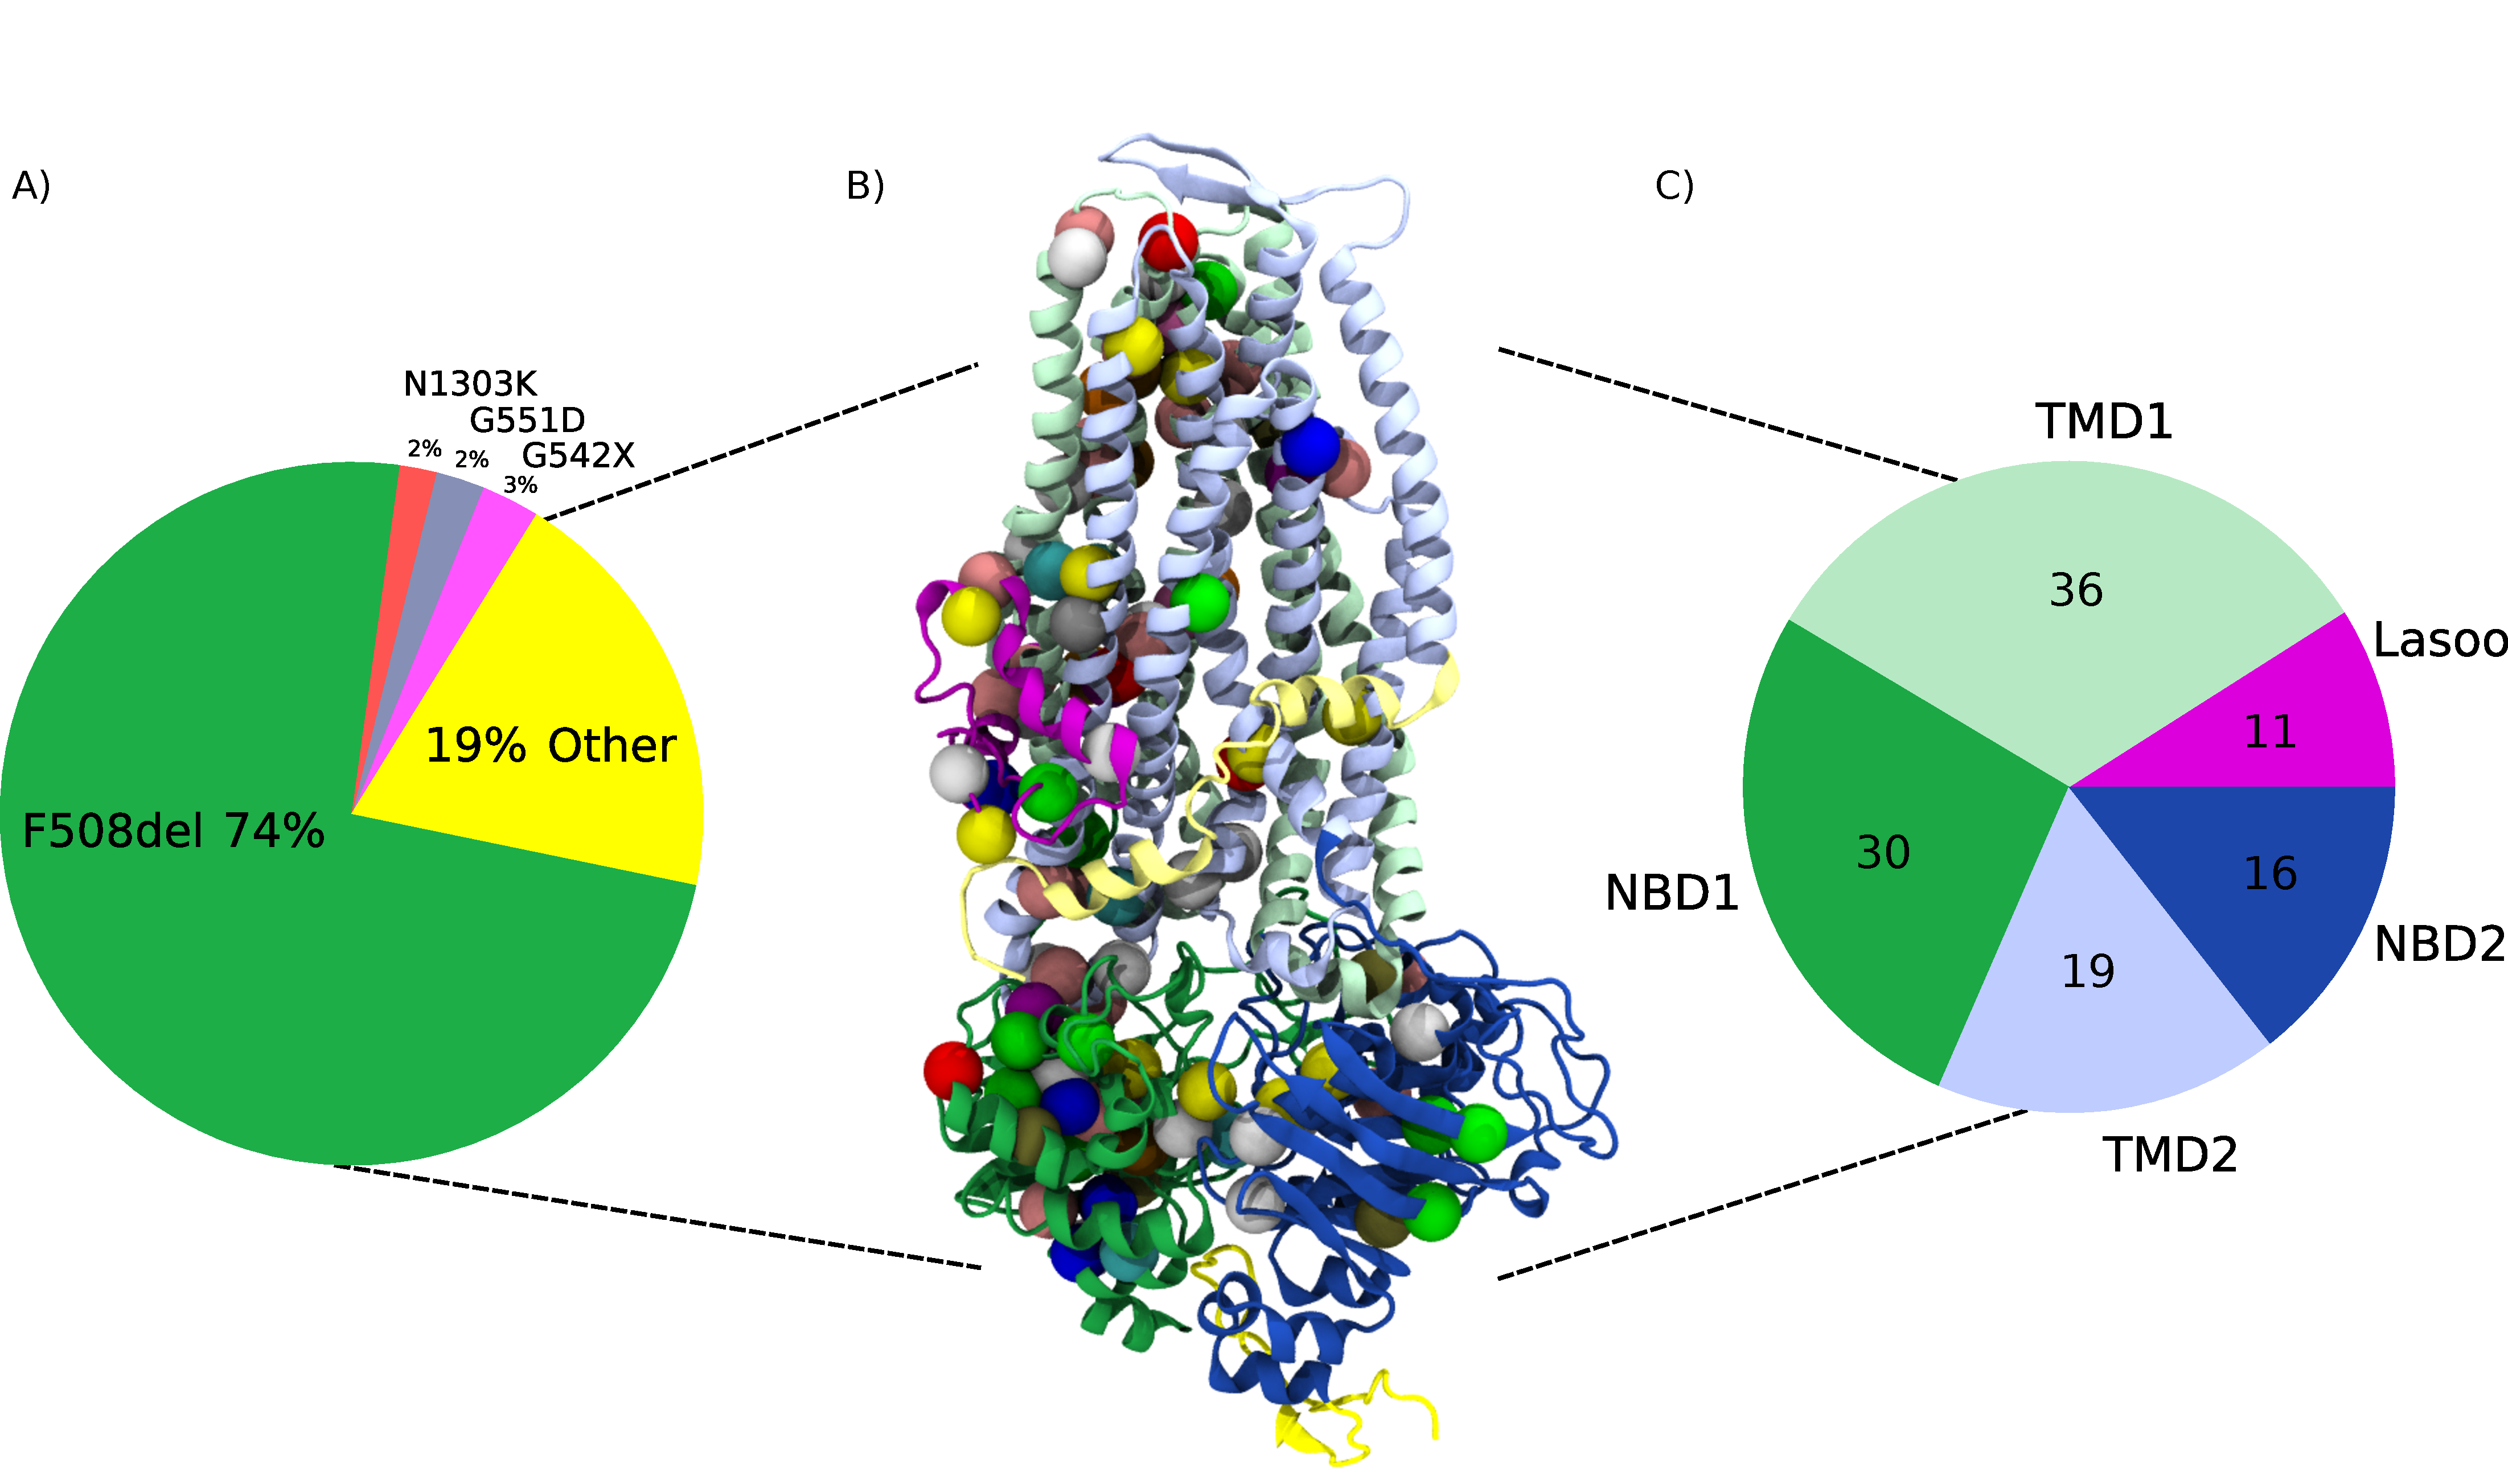
\includegraphics[width=\textwidth]{figures/alleles_pie_chart.pdf}
	\end{center}
	\label{CFTR_structure_domains}
	\captionsetup{singlelinecheck = false, justification=raggedright}
	\caption[Rare Mutations Occur in All parts of the CFTR Protein] {\textbf{Rare Mutations Occur in All parts of the CFTR Protein}}{A) The reported frequency of individual disease causing alleles in the CFTR2 database. At the time of writing there are 401 recorded disease causing alleles. A patient with CF will carry two of these mutations. The numbers here include all kinds of mutations, not just missense mutations. CF is a recessive gene so a patient patient will have defective copies of the CFTR gene in their genome. 1 in 25 people of Northern European descent are a carrier for CF and are themselves at increased risk for many health problems \cite{ioannou2014, miller2020}. B) The location of all 111 known disease causing missense on the CFTR protein itself. In addition to those visualised here there are many of variants of unknown significance (VUS). C) The number of CF causing missense mutations in the different domains of the CFTR protein. TMD1 and NBD1 have the highest concentration of disease causing mutations. Likely due to the former's role in ion permeation and the latter's role in gating \cite{cftr2}}. There are no CF causing missense mutations in the C-terminus or the R-domain. As more patient registries are updated across the world it is likely that more CF causing mutations will be discovered in the future.  
\end{figure}


\begin{itemize}
	\item \textbf{Class I} No functional protein. Under these mutations no protein is transcribed due to either problems with the transcription of mRNA or a premature stop codon truncating protein synthesis early, meaning the resulting peptide is missing key domains. 
	\item \textbf{Class II} Folding defect. These mutations cause the translated peptide to misfold into the incorrect tertiary structure. This can inhibit the protein's journey as it is trafficked to the cell membrane, its function while once it is there or its functional life time at the surface. 
	\item \textbf{Class III} Impaired Gating. Here the mutation inhibits the ability of the protein to transition from the closed to the open state. 
	\item \textbf{Class IV} Decreased Conductance. These mutations cause a barrier in the energy landscape of the CFTR chloride conductance pathway.
	\item \textbf{Class V} Less Protein Expressed.  
	\item \textbf{Class VI} Decreased Lifetime

\end{itemize}

Although useful, in reality this paradigm struggles to reflect the fact that a mutation can belong to multiple categories to different levels due to different modes of pathogenesis. Through our molecular simulations we can see that in reality CFTR modulators are capable of treating several different mutations with very different molecular fingerprints. We will break down this paradigm into more molecular detail in chapter \ref{chap:conclusions}

%FIGURE demonstrates how each of the canonical classes at the molecular level is broken down into many sub classes and a mutation might belong to one of many of these subclasses. Structural biology paradigms and \textit{in silico} modelling can help classify mutations into these different classes. In combination with wet lab assays we can understand which classes of these molecular defects are most effectively treated with specific drug regimens. Our computational microscope is helping choose treatments for patients at the atomic level. 

\section{Patients with Rare Rutations Struggle to Access Modulator Therapy}
We will explore the mechanism behind CFTR modulators shortly. However, first we should outline the specific, pragmatic motivations for the molecular modelling carried out in this thesis. Roughly 50\% cases of Cystic Fibrosis are caused by a homozygous mutation, $\Delta$F508, and 90\% of patients carry at least one copy of this mutation. At the time of writing, many jurisdictions such as Australia, the USA and the EU have approved a triple therapy known as Trikafta which can improve the outcomes for patients with one copy of $\Delta$F508. . However, this leaves a significant part of the CF afflicted population without access to this life saving medication \cite{}. The work in this thesis demonstrates that a larger section of the CF population is likely to respond to modulators, particularly those carrying missense mutations.

The treatment of rare mutations has particular importance in CF, not only will patients be left behind, but in fact by studying rare mutations outcomes can be improved for all CF sufferers. Potentiator class drugs were discovered by the study of a rare mutation G551D, through high throughput screening \cite{vangoor2009}. By studying rare mutations we can gain a more complete picture of the disease and so improve therapies for everybody. This is particularly important as CF is uncovered in regions where it is genetically rarer and so patients in these regions are more likely to have rare, due to the spectrum of CFTR genotypes \cite{singh2015,zheng2017,ni2022}. As patient registries are set up in these populations, more rare forms of CF are likely to be discovered. Many of these regions do not train physicians in the treatment of CF because of the disease's relative rarity, leading to poor patient outcomes \cite{}. The more modulators are available the cheaper individual drug costs will become and the more options patients will have to personalise their treatment.

Patients with rare forms of CF are more likely to be in countries where CF is already quite rare \cite{zheng2017}. Patients on modulators have significantly different clinical outcomes even between those with the same genotype. Determining the reason for this would open the door to the development of complimentary therapeutics. 

\section{CFTR is a Unique ABC Transporter}

\begin{figure}
	\label{ABC_diversity}
	\begin{center}
	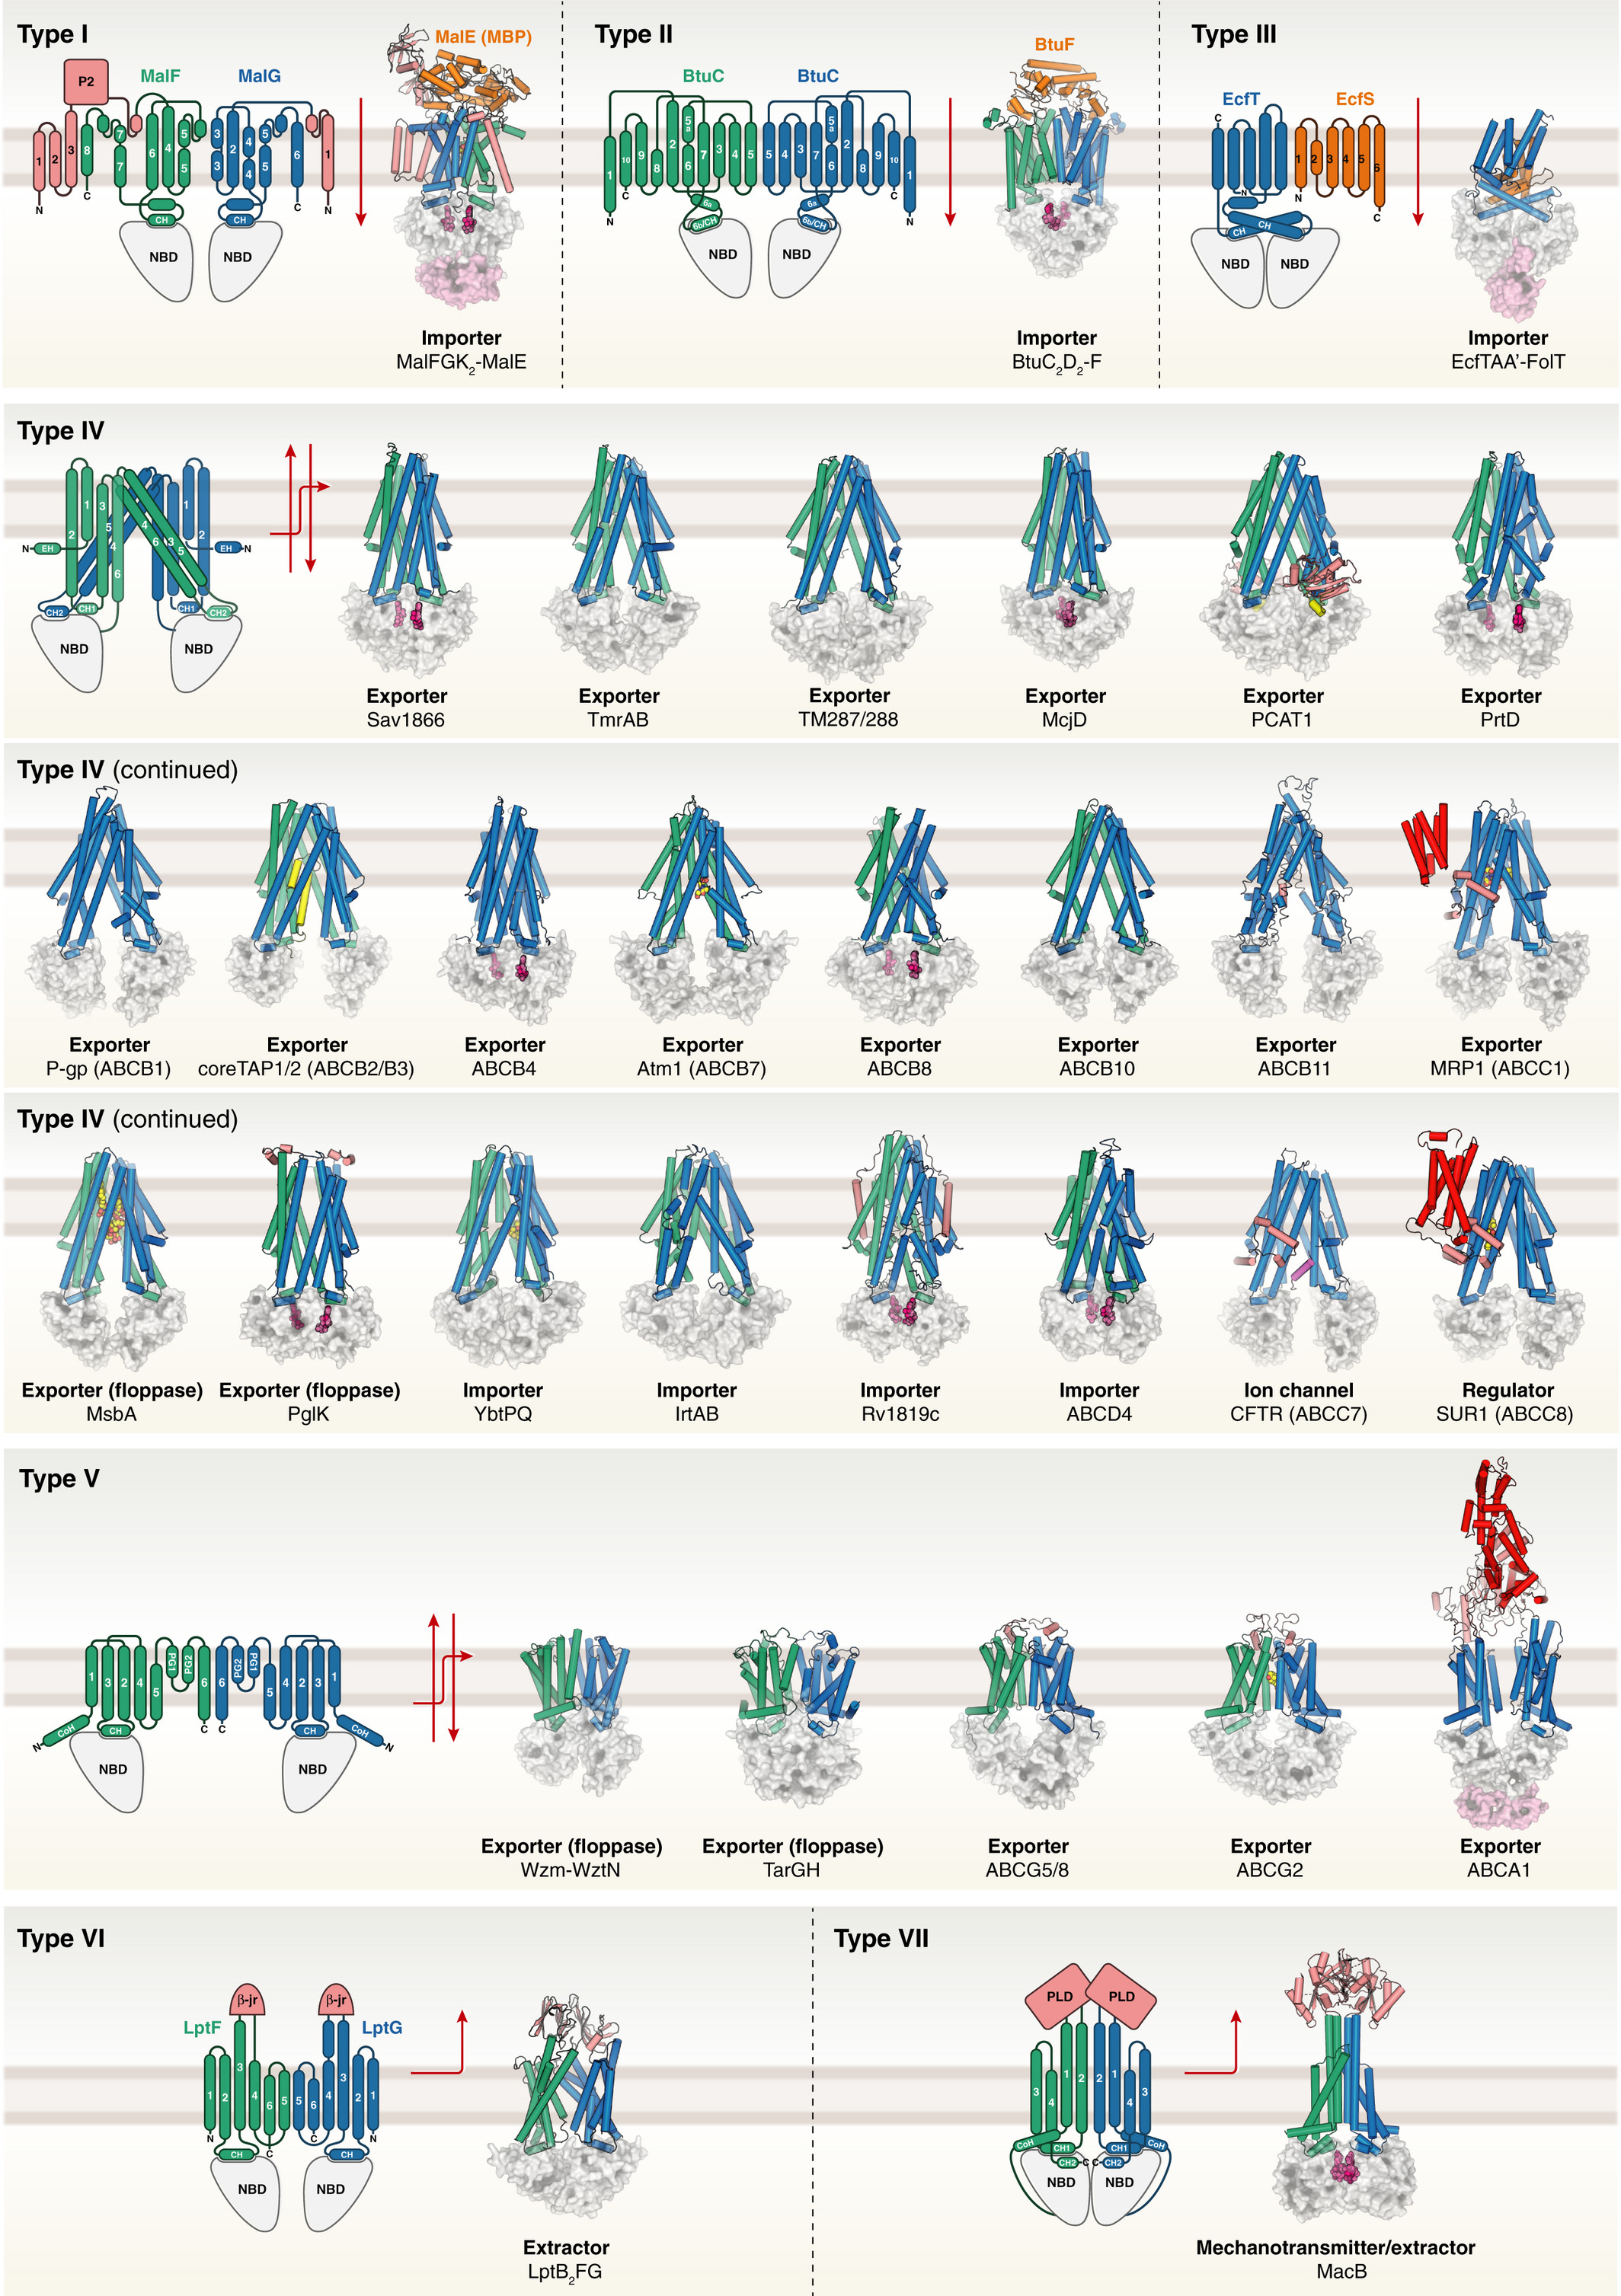
\includegraphics[width=\textwidth]{figures/ABC_classification.jpg}
	\end{center}
	\captionsetup{singlelinecheck = false, justification=raggedright}
	\caption[CFTR Structure] {\textbf{CFTR Structure}}{The structural diversity of ABC transporters. Structures are classified based on the organisation of their TMDs source \cite{thomas2020}.} 
\end{figure}
ATP-Binding Cassette (ABC) transporters are an intriguing super family of proteins. On the whole, they transport substrates by using a combination of phosphorylation energy from ATP hydrolysis. These can be diverse substrates such as lipids or small molecules. Their structural diversity can be seen in figure \ref{ABC_diversity} reflecting their array of functions. 

CFTR is unique, as it is not a transporter, but rather an anion \textit{channel}. The kinetic energy of the ATP is not used to translocate substrate across the membrane but rather simply used in the regulation of the gating cycle. There is ongoing debate about how closely hydrolysis is coupled to the diffusion of ions \cite{}. Chloride, bicarbonate and other anions are able to passively diffuse through the channel. This evolutionary misappropriation of a transporter to a "leaky channel" is perhaps the reason so many mutations can create a non-functional protein \cite{depristo2005,linsdell2018}.
CFTR belongs to a super family of proteins known as ATP Binding Cassette Transporters,  many of these proteins perform active transport across cell membranes. The substrates they transport can vary, including lipids and drug molecules. Proteins in this family share a common motif known as Nucleotide Binding Domains (NBDs). These domains act as ATPases, accelerating the hydrolysis of ATP. The energy from hydrolysis is then transferred into the protein in order for it to pump its substrate against a concentration gradient. 


\section{Modulators Act on CFTR to Restore its Function}
Since CF is caused by malfunctions of the channel it makes sense to pursue CFTR as a drug target. Through high throughput \textit{in vitro} screening several four compounds have been developed which act directly on CFTR to rescue its function. These fall into two classes. Correctors, which aid CFTR to fold into the correct state and potentiators which help the channel reach the fully open state once it has folded correctly and integrated into the membrane. Emerging evidence suggests that specific genetic defects may be optimally rescued by specific combinations and doses of both correctors and potentiators compounds \cite{}. Recently, cryo-EM structures of many of these compounds in their bound state have been released \cite{liu2019, fiedorczuk2022}. In addition to several \textit {in vitro} biophysical experiments to determine the precise mechanism of action and binding site of these compounds.

What is remarkable is that modulators they have demonstrated promise in relieving not just the most acute symptoms of CF (lung function), but there is also evidence that they may be able to aid in treating or even relieve deleterious complications such as bacterial infections and CF related diabetes  shown to aid in the relief of CF related complications such as bacterial infections or CF related diabetes symptoms \cite{gaines2021,lopes-pacheco2020, yi2021}. This highlights the importance of treating the root cause of a disease like CF.

\subsection{Correctors}
The mechanism of action for corrector compounds appears to be to bind to to a pocket between TMH1 and TMH3. Circular dichromism \cite{greenfield2006} and fluorescence experiments found that an isolated construct of TMH3 and TMH4 were more likely to fold correctly in the presence of corrector compounds. Later cryo-EM structures discovered high resolution electron density in the pocket in the shape of the drug compounds \cite{fiedorczuk2022}, confirming this hypothesis. 

In combination this is strong evidence for the precise mechanism of action for corrector compounds. Further work will aid in the creation of new compounds to refine our exploitation of this mechanism.

\subsection{Potentiators}
Potentiator class drugs bind to CFTR in order to smooth the transition to the fully open, conducting conformation \cite{yeh2017}. This increases the total number of open CFTR ion channels at any one time and helps to balance osmotic pressure over the epithelium.

There is some uncertainty surrounding the precise mechanism of potentiators drugs, with different studies discovering different binding sites via mutagenesis and other methods \cite{yeh2019, liu2019, laselva2021}. Evidence strongly supports their findings that potentiators bind directly directly to CFTR in order to increase the likelihood that it occupies a conducting state, with some potentiators rescuing CFTR with picomolar affinity \cite{csanady2019}. Controversy arises surrounding \textit{where} these drugs are acting to rescue CFTR. There are are cryo-EM structures which show the drugs bound to the TM8 hinge region \cite{liu2019}. However, there are some controversies surrounding the structure in which the drugs are bound in this study which we will discuss in \ref{chap:conclusions}. \textit {In vitro} experiments studying drug binding kinetics suggest at least two membrane facing binding pockets \cite{csanady2019}. 

GLPG1837 has not been approved in a clinical setting. \textit {In vitro} experiments suggest that it is more efficacious even though it has lower affinity for CFTR binding (CITATION NEEDED). This would indicate that the highest affinity binding pocket does not produce the greatest modulation. More work is needed to resolve the mechanism which results in the clinical effectiveness of these drugs.  

These drugs are clinically efficacious \cite{VanGoor2014} on several mutants with some curious exceptions like N1303K. I suggest the following mechanism for their action. I suspect a similar analogy exists for the action of the correctors. WT-CFTR exhibits a natural landscape with kinetic barriers in the transition between the closed and open states. A gating class mutation to CFTR will introduce a kinetic barrier in the pathway of this conformational transition. What these drugs do is reduce a barrier in the existing conformational landscape of CFTR. This compensates for the barriers introduced by the mutation. 

This provides a rationale for why it appears possible for diverse range of molecular defects to be treatable by these small molecules. In our work we've found that the atomic nature of the defects introduced by each mutation varies widely, what is interesting is that experiments in \textit{ex vivo} models have shown that these drugs treat a variety of different defects. The classification of classes of defect is outdated, really there are as many classes as there are mutations.

\subsection{Read Through Compounds}
Roughly 10\% of mutations result in a premature stop codon in the mRNA of the CFTR gene so synthesis is stopped early. Since there is no full length CFTR protein synthesised by the cells carrying this mutation, potentiators and correctors are unable to assist. This has lead to the need to develop a class of drugs known as read through compounds which allow the continued synthesis of the protein past the premature stop codon \cite{}. At the  time of writing no read through compounds have been clinically approved. Since correctors and potentiators also act on WT-CFTR it is likely that modulator therapy would be given in combination with read through compounds as a supplementary treatment \cite{}.

\section{Patient Derived Organoids as a Pre Clinical Model for Assessing Modulator Efficacy}
Similar to how we took the motions of interacting atoms in chapter \ref{chap:methods} to understand a biomolecular system, clinicians and cell biologists are increasingly capable of measuring the behaviour of a subset of cells to predict the outcome for a patient. Pre-clinical models can be used for testing what might produce the best clinical outcomes for the patient. For the case of Cystic Fibrosis researchers have begun to take samples of epithelial stem cells of patients with the disease and grow those samples into tissues which mimic the function of the entire organ\cite{depoel2020}. This is possible in the epithelium due to a population of adult stem cells which maintain the ability to differentiate into a variety of cell types (a property known as pluripotency). 

Primarily, these epithelial stem cells are taken from the nasal passages of patients or from rectal biopsies. These samples can then be grown into organoid models of the lung or gut respectively. 

Adult stem cells in the epithelium are preferable because other sources of stem cells such as induced pluripotent stem cells (iPSCs) require complex, time consuming protocols to grow into fully developed organoids. Already the differentiation and expansion of epithelial samples takes a month \cite{}.

In the case of CF this technology allows the construction of a scalable, patient specific platform where a patient's own tissues can be tested to determine the best treatment for them. These pre-clinical models will allow more patients in the heterogeneous set of disease causing mutations to access modulators. This has given rise to an exciting prospect of a practice known as theratyping, enabling clinicians to make a personalised choice of which drugs which drug regimen will best serve a patient \cite{clancy2019, wong2022, wong2022a, ciciriello2022}. This thesis demosntrates that integration of \textit{in silico} simulations into this process can further the capabilities of these pre-clinical models.

%One limitation of these organoid platforms is the lack of an inflammatory response since no immune cells are present in the tissue culture. 
The response of the patient's epithelium is characterised using a few \textit{in vitro} assays which we will briefly discuss below. 

\subsection{Forskolin Induced Swelling to Assess CFTR Function}
Forskolin Induced Swelling (FIS) assays have been used to characterise the patient specific response of a patient's organoids to a drug regimen \cite{dekkers2013}. When epithelial cells are exposed to a chemical known as Forskolin they begin to rapidly produce cyclic AMP (cAMP, a precursor to ATP in a cell) \cite{}. This allows the down stream activation of CFTR ion channels, causing the organoids themselves to swell. This swelling allows cell biologists to easily quantify the activity of CFTR within a patient, in a variety of conditions.

\subsection{Measuring Cilia Beating Frequency Allows Personalisation of Treatment}
The lungs are covered in cilia which fluctuate or "beat" in order to clear mucus and other particles in the respiratory tract \cite{mitchison2010, bustamante-marin2017}. One of the most characteristic symptoms of patients with Cystic Fibrosis is the build up of mucus around the epithelium. This causes cilia to collapse, meaning they cannot move \cite{}. By measuring the frequency at-which the cilia beat one can determine whether a modulator regimen will produce an optimal clinical outcome.

\subsection{Electrophysiology}
Since CFTR is an ion channel, measuring its electrical activity is a direct way to assess its function. For single channel studies this is done with a patch clamp. However, this does not give an assessment of the whole epithelium. Often the whole organoid is used as a patch and put in an Ussing chamber. By blocking other ion channels such as ENAC a clear picture of CFTR function can be measured in order to create a pre-clinical model for a specific patient.

\subsection{Western Blotting to Assess CFTR Trafficking}
The above methods may be able to properly quantify gating class mutations but they will struggle to assess the amount of CFTR at the cell surface. For this we employ .
